\chapter{Logistic Regression}

The objective here is discussing the \textbf{Logistic regression} model which is used for \textbf{binary}, and also, \textbf{multiclass classification}. We will start from the hypotesis $h_\theta(x)$ used in the case of regression, we will analyze the aspects which will be maintained of it, and also the cons. 

\section{Classification vs Regression}
Coming back for a while to the problem of \textit{tumor classification}, suppose that a linear hypotesis can be used in order to separate the data. The comprehension of this concept is aided by the following figure: 
\begin{figure}[h]
    \centering
    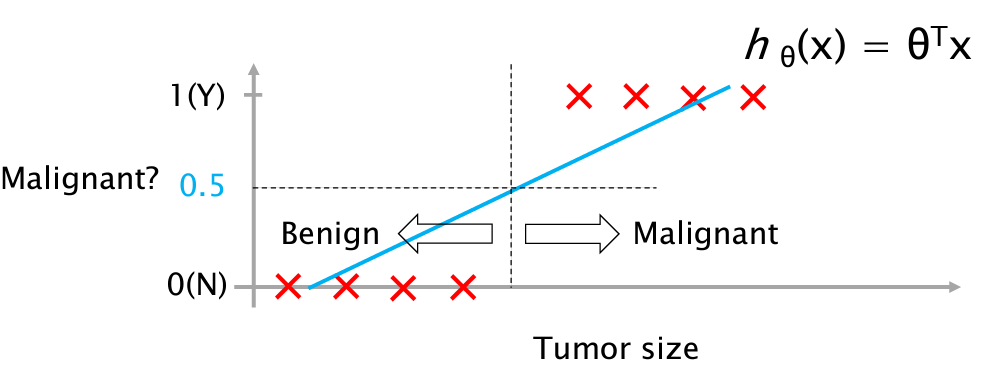
\includegraphics[scale=0.5]{img/Class_vs_Reg.png}
    \caption{Classification with linear hypotesis}
\end{figure}
The hypotesis $h_\theta(x)$ used in order to separate the two class is the line showed in blue. Since here we are not in the case of prediction of a continuous value, we have to find a way for shrink all possible output from the hypotesis in two values (Positive/Negative). At this point an idea could be using a threshold according which you can separate data from the two classes, that is:
\begin{equation} \label{eq:criteria}
    y=\begin{cases}
        1&\text{if} \ h_\theta(x)>0.5\\
        0&\text{if} \ h_\theta(x)\le{0.5}
    \end{cases}
\end{equation}
This appproach seems to work, until we do not change the data used for building the model. Let us consider, for example, the following scenario:
\begin{figure}[h]
    \centering
    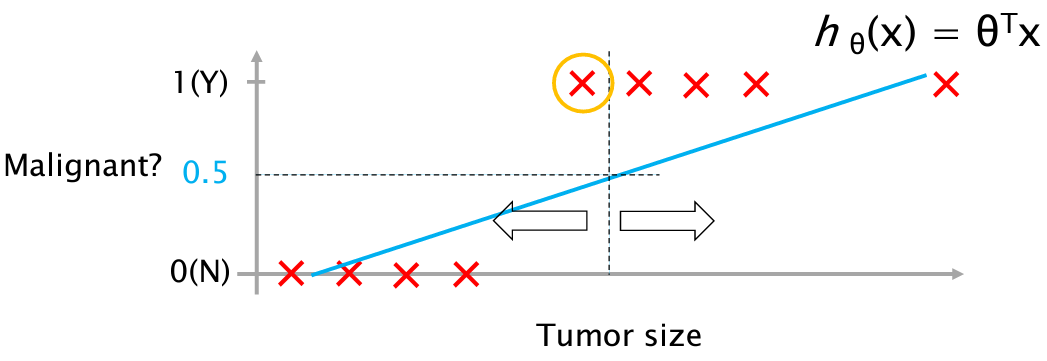
\includegraphics[scale=0.5]{img/Class_vs_Reg2.png}
    \caption{Effect of changing the dataset}
\end{figure}
It appears quite evident that one of the data for which we know that belongs to the positive class, is classified as negative.\\
This is not the only problem: we want that the predicted output\footnote{
    Later we will call it $\hat{y}$, for comparing it to the true output $y$.
}, that is the hypotesis is between 0 and 1, despite the fact of using a threshold this is not satisfied, since a linear function is \textit{unbounded}. At this point our reasoning leads to the formulation of the following two issues:
\begin{enumerate}
    \item A \textit{linear hypotesis} is not suitable for a classification problem, the performances would be awful also on the training set; 
    \item It is required that $$ 0 \le h_\theta(x) \le 1$$ this is not happening in the cases a linear hypotesis is employed.
\end{enumerate}
These are the main points that leads to the \textit{correct formulation} of \textbf{logistic regression}\footnote{
    The name \textit{logistic} is related to the fact that we are solving a dicotomic/binary classification problem.
}.

\section{Logistic regression}
The main concept behind \textit{logistic regression} is using a nonlinear function that saturates the hypotesis between 0 and 1. Basically we have to apply such a function which we will call $g(z)$ to the linear $\theta^T{x}$, such a function is called \textbf{sigmoid} or \textbf{logistic function}. It is depicted in the following and its expression is:
\begin{equation}
    g(z)=\frac{1}{1+e^{-z}}
\end{equation}

\begin{figure}[h]
    \centering
    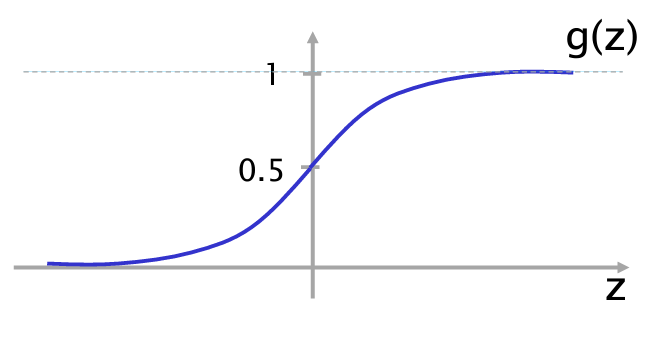
\includegraphics[scale=0.7]{img/logit.png}
    \caption{The logistic function $g(z)$}
\end{figure}

The output of such an hypotesis can be interpreted as \textit{the probability that the output y=1 on a given input x}, for example in the case of tumor classification a value of 0.7 of the hypotesis results in a prediction that for 70\% the given tumor (with its feature is malignant). In order to be mathematically formal we can say that 
\begin{equation}
    h_\theta(x)=P(y=1 | x; \ \theta )
\end{equation}
which is read "the probability for the output $y$ to be 1, given $x$, parametrized by $\theta$. Clearly, at the opposite we can compute
\begin{equation}
    P(y=0 | x; \ \theta) = 1 -P(y=1 | x; \ \theta )
\end{equation}
Here we can stick to the fact of having a threshold. More specifically, we use as an hypotesis $g(\theta^T{x})$ and we can use the criterion used in (\ref{eq:criteria}). Moreover for the particular function  $g(z)$ it is used we can say that, given the features $x$ then it is classified as positive if $\theta^T{x}\ge0$ or negative if $\theta^T{x}<0$, since the counterimage of 0.5 through $g(z)$ is equal to 0, as showed in the following figure.

\begin{figure}[h]
    \centering
    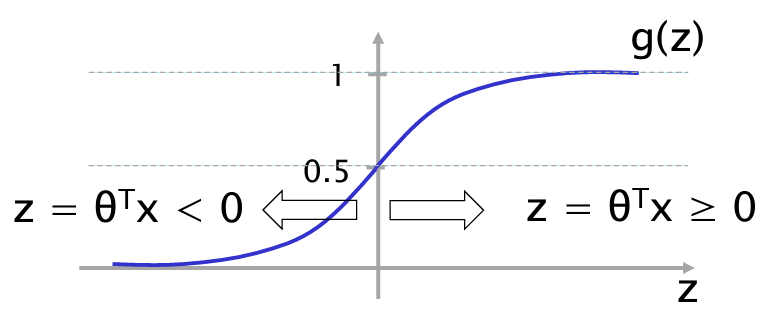
\includegraphics[scale=0.7]{img/logit2.png}
\end{figure}

It appears clear that the linear combination $\theta^T{x}$ is a (linear) \textbf{decision boundary} since it provides us with the information of having a positive or negative record. It is useful to give an example of this fact: 

\begin{figure}[h]
    \centering
    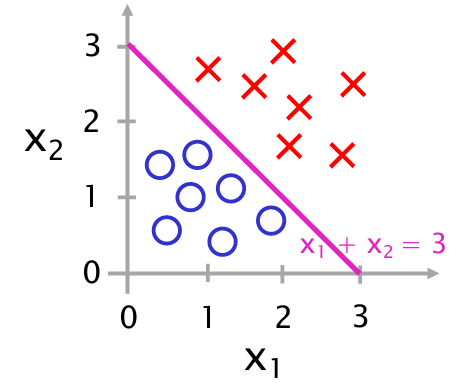
\includegraphics[scale=0.7]{img/decision_boundary1.png}
    \caption{Decision boundary}
\end{figure}

\noindent
Suppose we trained the model and the parameter theta resulted in being $\theta=[-3\  1 \ 1]^T$, this is the same to say that we assign \textit{positive class}to records with feature $x_1, x_2$ such that $\theta^T{x}$ is greater or equal than 0, negative class otherwise. Then, I can completely remove the record from the dataset and using such a decision boundary for doing classification. There are some cases in which due to the distribution of the data of each class, it is not possible to separate them with a linear decision boundary. In that case higher order nonlinear functions (eg. polynomials) must be used.

\section{Cost function for logistic regression}
We have seen in the former chapter about linear regression that a cost function is introduced to be minimized in order to find the parameter $\theta$ which are the best for our model.\\
In case we had a regression problem to be solved the functional $J(\theta)$ (Square Error) was a convex one, if we stick to the use of a sigmoidal function (and it is a proper choice for classification) the \textit{Square Error functional} becomes a non-convex one, so that the Gradient Descent Algorithm is not converging to a global minimum. What is changed for logistic regression is the \textbf{Loss function} associated to a single training sample. A particularly clever choice is the following:
\begin{equation}
    \text{Loss}(h_\theta(x),y) = \begin{cases}
        -\log(h_\theta)&\text{if} \ y=1\\
        -\log(1-h(\theta))&\text{if}\ y=0
    \end{cases}
\end{equation}

\begin{multicols}{2}

    \begin{center}
        \centering
        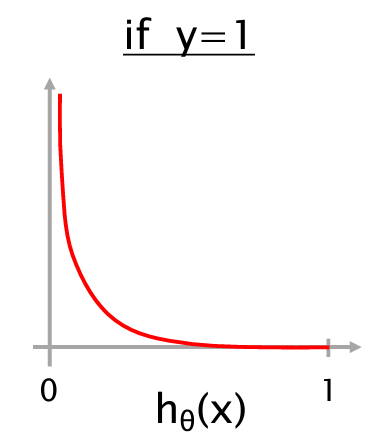
\includegraphics[scale=0.7]{img/Loss_y1.png}
    \end{center}
    \newcolumn
    \begin{center}
        \centering
        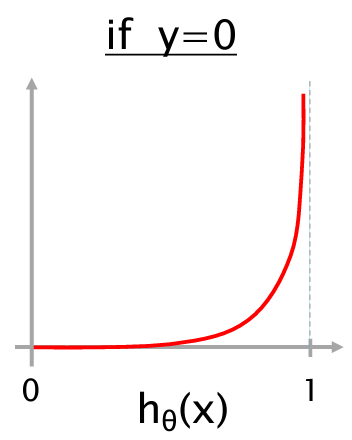
\includegraphics[scale=0.7]{img/Loss_y0.png}
    \end{center}
\end{multicols}

\noindent
Since the Loss function must penalize the objective to be effective in case the effective output is $y=1$ and the hypotesis (formulated with those parameters) would give 0, then the cost is very high. On the contrary a positive hypotesis with an actual output of $y=0$ will give to the functional a very high contribution, resulting in an high penalization (keep in mind that the functional must be minimized). This concept has a quite intuitive explanation as we have seen. \\
It would be useful having an \textit{overall functional} and with the aim of obtaining it, we badly exploit the fact that the output is logistic. In particular: 
\begin{equation}
    \text{Loss}(h(\theta),y)=-{\color{red}y} \log{h_\theta{(x)} - {\color{red}(1-y)}\log{(1-h_\theta(x))}}
\end{equation}

\noindent
The cost function coming from such a loss function is the following and it is denoted as \textbf{Binary cross-entropy cost function}:
\begin{equation} \label{eq:cross-entropy}
    J(\theta)=
    \underbrace{-\frac{1}{m}\sum_{i=1}^m \bigg[
        -{\color{black}y^{(i)}} \log{h_\theta{(x^{(i)})} - {\color{black}(1-y^{(i)})}\log{(1-h_\theta(x^{(i)}))}}
    \bigg]}_{\textsf{\color{orange}BINARY CROSS-ENTROPY COST FUNCTION}}
\end{equation}

\section{Training logistic regression}
Given the cost function (\ref{eq:cross-entropy}), we minimize it by using gradient descent algorithm, given an unknown $x$ the output is provided by using the hypotesis 
\begin{equation}
    h_\theta(x) = \frac{1}{1+e^{-\theta^\textsf{T}{x}}}
\end{equation}

\noindent
The algorithm of gradient descent follows the same step as in \textit{linear regression}, what is changed is the shape of the hypotesis $h_\theta(x)$.

\section{Multiclass classification}
Suppose we want to do a multiclass classification, for example for tagging mail as \textbf{SPAM, WORK, FRIENDS...} Can we use logistic regression in order to carry out such a task? The answer is YES, but with some modifications. In the sense that we can reformulate the problem in \textit{one class against the others}. The steps are the following: (A) We train a logistic regression classifier $h_\theta^{(i)}(x)$ in order to predict $P(y=i|x;\ \theta)$ for each class $i$. On a new input the prediction is done as follows:
\begin{equation}
    i=\arg\max_{i} h_\theta^{(i)}(x)
\end{equation}
where $i$ is the $i$-th class. Is this a good idea for a multiclass classification? Not so much! In the sense that the computational load grows of a factor $n$, with $n$ the number of classes. 

\section{Overfitting and Regularization}
In building a predictive model, there are usually two problems which we want to avoid: \textbf{underfitting and overfitting}. In the former case, provided that there are a small number of features, the learned hypotesis will not fit properly the training set. We can also say that there is an \textbf{high bias} in the data. In the latter case (overfitting) the learnt model has got excellent performances on the training set, in the limit case $J(\theta)=0$, but \textit{fails to generalize new examples}, in this case there are \textit{too many features}, so there is an \textit{high variance} in the data. \\
The configuration which is in the middle is the so-called \textit{just right}, and it is the one we want to reach aiming to have a good model. 

\begin{figure}[h]
    \centering
    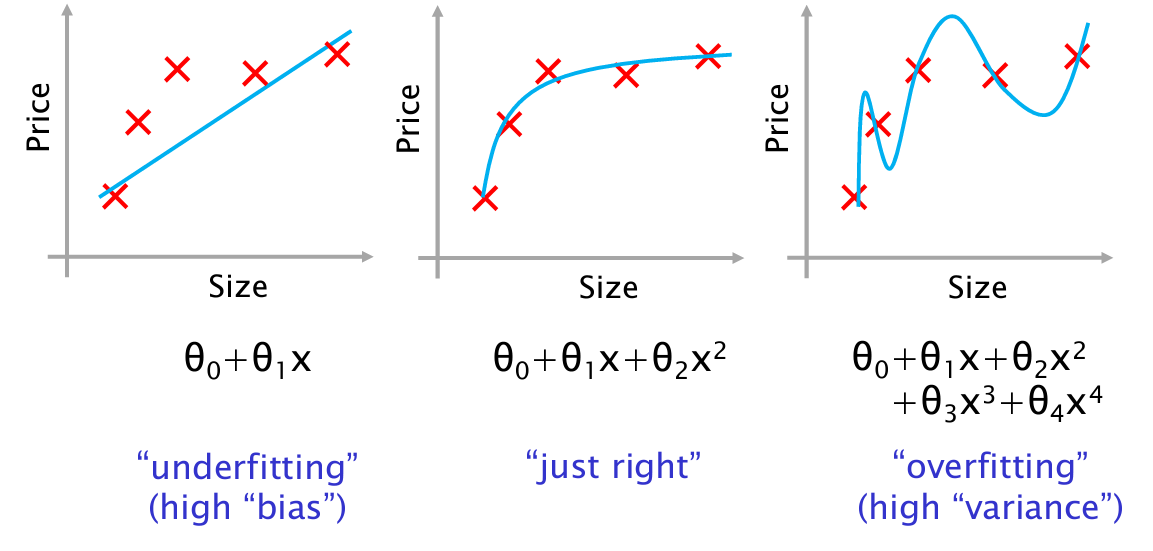
\includegraphics[scale=0.5]{img/over_under.png}
\end{figure}

\noindent
\textbf{What are the solutions for avoiding overfitting?} The first way is to reduce theb number of features the algorithm use for building the model (some techniques as PCA\footnote{
    PCA $\to$ Principal Component Analysis
} and LDA\footnote{
LDA$\to$ Linear Discriminant Analysis} can be used). Another way is introducing in the cost function a \textbf{regularization term}, its main purpose is to reduce the magnitude of the $\theta_i$ while keeping all the features. The regularization term acts directly on the parameters and it is proportional to the number of features. Using the regularization, simpler models can be obtained reducing the problem of overfitting the data. Let us consider for example the \textit{Square-error cost function}, when regularization is used it becomes:
\begin{equation} \label{eq:square_reg}
    J(\theta) = \frac{1}{2m} \sum_{i=1}^{m} (h_\theta(x^{(i)})-y^{(i)})^2 + \frac{\lambda}{2m} 
    \sum_{j=1}^{n} \theta_{j}^{2} 
\end{equation}
It is remarkable that the square-error cost function works on the $m$ training examples, while the regularization term\footnote{
    Do not confuse yourself with the \textit{normalization} which is done on the data
}interests directly the parameter of the model. The parameter $\lambda$ becomes another hyperparameter and we refer to it as the \textit{regularization parameter}. Clearly the optimization algorithm (Gradient Descent) must be updated accordingly. We also call the regularization in (\ref{eq:square_reg}) the $\ell_2$-regularization since it involves the $\ell_2$-norm definition. In the field of optimization models also the $\ell_1$-norm is considered, but in this case alternative techniques must be employed since the $\ell_1$-regularization makes the functional a non-differentiable one. Different algorithm, like ISTA and FISTA, have been developed in order to deal with such a type of optimization problem.